%Kelompok Memory Allocation
%Arjun Yuda Firwanda
%Dezha Aidil Martha
%Dwi Septiani Tsaniyah
%Muh.Rifky Prananda
%Yusuf Al-Qordhawi

Memory Allocation

\section {Memory Allocation}

\subsection {Pengertian Memori}

Memori adalah pusat dari operasi computer. Memori sebagai tempat penyimpanan dan dapat menyimpan file atau program dimana file tersebut tergantung ruang atau space penyimpannya di dalam komputer. Memori sabagai tempat penyimpanan yang harus di dijaga dengan sebaik mungkin agar terhindar dari virus atau file yang dapat merusak program atau fie yang disimpan.

\begin{figure}[ht]
\centerline{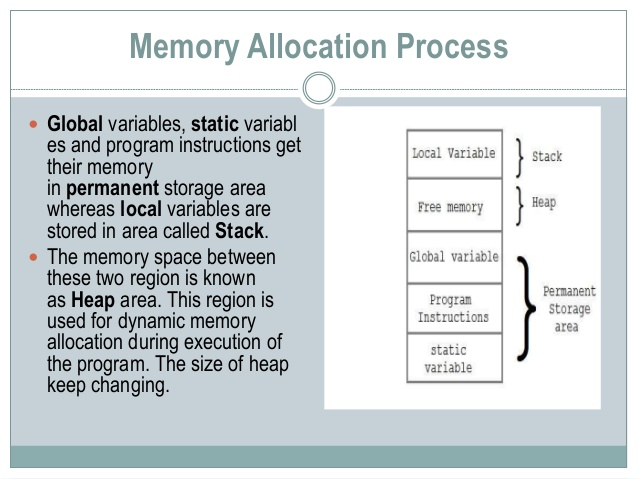
\includegraphics[width=1\textwidth]{figures/memory_allocation.jpg}}
\caption{gambar memory allocation.}
\label{memory allocation}
\end{figure}


\subsection {Fungsi Allocation Memori}


Manajemen memori merupakan salah satu bagian terpenting pada sistem operasi. Memori sangat perlu dikelola dengan sebaik-baiknya agar :

1. Utility CPU akan meningkat.
2. Data dan instruksi akan diakses dengan cepat oleh CPU.
3. Tercapai efisiensitas dalam pemakaian memori.
4. Transfer data memori utama ke/dari CPU lebih efisien.
5. Mengelola informasi. 
6. Mengalokasikan memori ke proses yang diperlukan. 
7. Mendealokasikan memori dari proses yang telah selesai. 
8. Mengelola swapping atau pagging antara memori utama dan disk.

Jenis memori ada 2 yaitu RAM dan ROM, RAM adalah Random Akses Memori yang isi penyimpanannya dapat diakses dalam waktu yang tetap. ROM adalah Read Only Memori adalah penyimpanan data yang permanen. sedangkan jenis-jenis memori eksternal ada 2 yaitu berdasarkan karakteristik bahan dan berdasarkan jenis akses data. Tentunya hal tersebut tergantung space dan ruang penyimpanan yang ada.

1. RAM

{figure}[ht]
\centerline{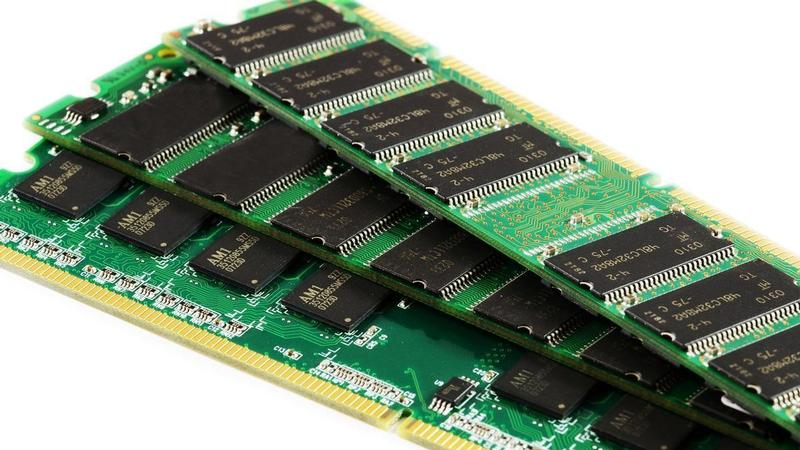
\includegraphics[width=1\textwidth]{figures/RandomAksesMemori.jpg}}
\caption{gambar RandomAksesMemori}
\label{RandomAksesMemori}
\end{figure}

2. ROM

{figure}[ht]
\centerline{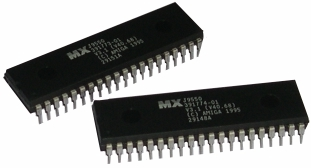
\includegraphics[width=1\textwidth]{figures/rom.jpg}}
\caption{gambar rom}
\label{rom}
\end{figure}


\subsection {Manajemen Proses}

A. Proses
Proses adalah sebuah program yang akan dieksekusi atau yang sedang belangsung. Sedangkan program adalah kumpulan instruksi yang ada di dalam program dengan bahasa yang mudah dimengerti system operasi. Proses berisi instruksi dan data. Program counter dan semua register pemroses, dan stack berisi data sementara seperti parameter rutin, alamat pengiriman dan variabel-variabel lokal.Sistem operasi menjalankan semua proses di sistem operasi dan mengalokasikan sumber daya ke dalam proses-proses yang sesuai dengan kebijaksanaan untuk memenuhi salah satu sasaran sistemnya itu sendiri. Abstraksi proses yaitu merupakan  hal yang mendasar dalam manajemen proses-prosesnya yang bejalan di sistem. Sistem operasi dalam mengelola proses ini dapat menjalankan operasi-operasi terhadap suatu proses.


B. Istilah yang terkait dengan Proses
Istilah Proses dapat dibagi menjadi dua, yaitu :

1. Multi Programming (Multitasking)
Multi Programming atau Multitasking adalah suatu istilah yang merujuk kepada metode banyak pekerjaan yang disebut proses, diolah menggunakan sumber daya CPU yang sama-sama bekerja.

{figure}[ht]
\centerline{\includegraphics[width=1\textwidth]{figures/multiprogamming.jpg}}
\caption{gambar multiprogramming.}
\label{multiprogramming}
\end{figure}


2. Multiprocessing
Multiprocessing adalah Kemampuan komputer menjalani tugas beberapa proses secara bersamaan dengan menggunakan teknologi berbasis multiprocessor.
Contoh : Rendering Video, Compress File, dan sebagainya.

{figure}[ht]
\centerline{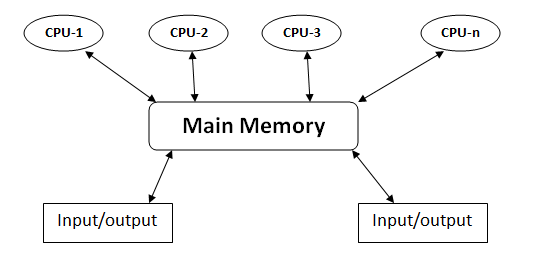
\includegraphics[width=1\textwidth]{figures/multiprocessing.png}}
\caption{gambar multiprocessing.}
\label{multiprocessing}
\end{figure}


C. Tipe-tipe Manajemen Proses

\begin{figure}[ht]
\centerline{\includegraphics[width=1\textwidth]{figures/manajemenproses.jpg}}
\caption{gambar manajemen proses}
\label{manajemen proses}
\end{figure}

a. Berdasarkan keberadaan swapping :

	1. Manajemen tanpa swapping.
		Manajemen memori tanpa pemindahan citra proses antara memori utama dan disk selama ekseskusi.
	
		\begin{figure}[ht]
		\centerline{\includegraphics[width=1\textwidth]{figures/manajemen tanpa swapping.jpg}}
		\caption{gambar manajemen tanpa swapping.}
		\label{manajemen tanpa swapping}
		\end{figure}


	2. Manajemen dengan swapping.
		Manajemen memori dengan pemindahan citra proses antara memori utama dan disk selama ekseskusi.

		\begin{figure}[ht]
		\centerline{\includegraphics[width=1\textwidth]{figures/manajemen swapping.jpg}}
		\caption{gambar manajemen swapping.}
		\label{manajemen swapping}
		\end{figure}


b. Manajemen Memori Berdasarkan Alokasi Memori

Terdapat dua cara menempatkan informasi ke dalam memori kerja

	1. Alokasi Memori (Contigouos Allocation)
		- Dalam alokasi memori berurutan, setiap proses menempati satu blok lokasi memori berurutan tunggal.
		- Keuntungan: sederhana, tidak ada rongga memori proses sekuensial yang tersebar dapat dieksekusi dengan cepat.
		- Kekurangan: memori yang sia-sia, tidak bisa dimasukkan saat tidak hadir satu blok memori yang cukup.

	2. Alokasi Memori yang Tidak Dihitung (Alokasi Tidak Berdampingan)
		- Program/proses ditempatkan pada beberapa sambaran tersebar, tidak harus dekat satu sama lain atau berurutan. Biasanya digunakan untuk lokasi memori virtual sebagai lokasi halaman-halaman.
		- Keuntungan: sistem dapat memanfaatkan memori utama lebih banyak efisien, dan sistem operasi masih bisa memasukkan protes kapan jumlah lubang memori cukup untuk memuat proses itu akan dieksekusi.
		- Kekurangan: membutuhkan kontrol yang lebih rumit dan begitu banyak memori yang tidak terpakai.

	Selain itu, ada 2 tipe manajemen memori yang digunakan, yaitu :
	a. Static Memory Management (Manajemen Memori Statis)
	b. Dynamic Memory Management (Manajemen Memori Dinamis)

Tipe manajemen ini memiliki Partition yang berbeda jenis, jumlah memori, penempatan/lokasi, dan ukuran yang diproses
oleh memori itu sendiri. Dari 2 tipe manajemen memori disebutkan terdapat perbedaan diantara keduanya yaitu :
a. Manajemen Memori Statis  tidaklah akan berjalan bersama karena berbeda jenis manajemen memori
b. Manajemen Memori Dinamis akan berjalan bersama karena kemiripan/kesamaan jenis manajemen memori.

\subsection {Manajemen Memori Pemartisian Statis}

Kondisi tanpa swapping :

a. Monoprogramming.
Monoprogramming manajemen yaitu memori yang paling sederhana di dalam sistem komputer hanya dapat mengijinkan satu sistem atau satu pemakai saja dengan berjalan pada satu waktu. Semua sumber daya sepenuhnya akan dikuasai oleh proses yang sedang berjalan.

b. Multiprogramming dengan pemartisian statis
Multiprogramming dapat dilakukan dengan cara pemartisian statis, yaitu memori dibagi menjadi beberapa bagian dengan sejumlah partisi tetap . pada partisi ini proses-proses ditempatkan.

1. MONOPROGRAMMING :

	1.hanya terdapat satu proses pada suatu saat, sehingga proses baru akan mempengaruhi kepada proses lama.
	2. semua memori hanya dapat di gunakan satu proses saja.
	3. pemakai hanya memusatkan kepada satu memori atau tape.
	4.suatu mesin di kendalikan oleh suatu program.

		MONOPROGRAMMING:

	- Masih digunakan untuk sistem kecil yaitu embedded system (embedded system) terpasang atau ditemukan di sistem lain.
	- Sistem tertanam menggunakan mikroprosesor kecil, seperti Intel 8051.
	- Sistem ini biasanya untuk mengendalikan satu alat menjadi umum kecerdasan (perangkat intelegent) dalam menyediakan fungsi tertentu. Karena hanya satu fungsi spesifik, dapat diprogram dalam mikroprosesor dengan memori kecil (1-64 Kb).

2. Memproses / mendistribusikan komputasi.

Pengolahan / komputasi terdistribusi adalah Bekerja semua pemrosesan data bersama dengan komputer.

Misalnya: komputer yang dirancang untuk tugas proyek

\subsection {Proses Status}

Ada 5 jenis status berbeda yang mungkin dimiliki oleh proses:

1. Baru, status yang digunakan ketika proses baru saja dibuat
2. Siap, yaitu status di mana proses siap untuk dilaksanakan pada giliran berikutnya
3. Menjalankan, yaitu status saat ini sedang dieksekusi oleh prosesor
4. Menunggu, yaitu status yang tidak dapat dijalankan saat prosesor siap / gratis, Status yang digunakan selama proses sedang berlangsung seperti proses I / O.
5. Dihentikan, yaitu status yang ditampilkan pada saat proses telah dijalankan

Berikut ini adalah proses 5 proses di atas menyatakan:

	a. Pertama dari Baru ke Siap
		Setelah status dibuat, statusnya akan siap untuk diproses lebih lanjut.
	b. Siap dijalankan
		Ketika memilih proses, sistem operasi memilih salah satu proses yang sudah jadi.
	c. Lari menunggu
		Suatu proses yang timbul dalam keadaan menunggu dari suatu proses yang membutuhkan sesuatu yang akan menyebabkannya menunggu. Permintaan ke sistem operasi biasa menjadi bentuk sistem layanan (dari program yang digunakan untuk operasi yang merupakan bagian dari sistem operasi) dan proses yang dapat digunakan oleh sistem operasi yang tidak dapat dilakukan secara langsung dengan sistem operasi. segera.

1) Lari ke siap
	Ini adalah proses berkelanjutan yang telah mencapai waktu maksimum yang mungkin untuk tidak terganggu. Ada beberapa alasan berbeda, yang tidak diterapkan di setiap sistem operasi. Sebagai contoh, sistem operasi memberikan tingkat prioritas yang berbeda ke proses yang berbeda, proses yang dianggap pertama.
2) Menunggu hingga siap
	Proses menunggu telah selesai mencari sumber daya, seperti file atau bagian memori virtual untuk digunakan atau telah diselesaikan selama proses lain untuk memberikan masukan atau telah selesai menunggu pesan lain.
3) Berlari sampai selesai (dihentikan)
	proses sedang dijalankan oleh SO ketika proses telah selesai atau dibatalkan. Ini terjadi karena proses self-making telah berhenti.

	PROSES CONTROL BLOCK/BLOCKED
	Struktur data yang dipakai oleh OS untuk mengelola suatu proses yaitu Process Control Blok. Hampir semua OS yang sudah modern telah memiliki PBC , tetapi terdapat struktur yang berbeda-beda pada setiap OS tersebut. Process Control Blok juga terdapat informasi tentang suatu proses yaitu sebuah tanda pengenal yang disebut process ID yang sangat unik dan menjadi nomor identitas, status process. Keutamaan di dalam suatu proses merupakan suatu nilai atau besaran yang menunjukan seberapa sering proses yang harus di jalankan oleh prosesor. Proses itu sendiri memiliki prioritas yang lebih tinggi , yang akan dijalankan secara terus-menerus atau dijalankan terlebih dahulu dibandingkan dengan proses yang berprioritas lebih rendah. Sebagai contoh , struktur data yang akan mengendalikan beberapa PCB yaitu process table. Tetapi bisa saja beberapa PCB disimpan pada daftar dalam waktu yang bersamaan . pada process table ini menggambarkan suatu sistem tersebut ketika OS menemukan setiap PCB melalui process ID.


\subsection {Multiprogramming dengan pemartisian statis}
Multiprogramming dapat dilakukan dengan pemartisian statis, yaitu memori dibagi menjadi beberapa sejumlah partisi tetap. Pada partisi-partisi tersebut proses-proses ditempatkan.


	MULTIPROGRAMMING

	Melibatkan banyak pemakai secara simultan sehingga di memori akan terdapat lebih dari satu proses bersamaan. Oleh karena itu dibutuhkan sistem operasi yang mampu mendukung dua kebutuhan tersebut.

	Melakukan dua aktivitas :
	- Proteksi memori dengan isolasi ruang-ruang alamat secara disjoint (terpisah).
	- Pemakaian bersama memori.

a. Multiprogramming Static Partitioning

	Batasi beberapa alasan:
	a. Sederhanakan pemogram.
	Pemrograman dapat memecah program menjadi dua atau lebih proses.

	b. Untuk dapat memberikan layanan interaktif kepada banyak orang secara bersamaan. Anda perlu memiliki lebih dari satu proses mememori untuk hasil kinerja yang baik.

	c. Biaya penggunaan sumber daya.
	Jika pada multiprogramming dan prosesnya diblocked (hanya DMA yang berfungsi) dan proses lainnya mendapat waktu pemrosesan penjatahan, lalu DMA dapat meningkatkan sistem mahal.

	d. Eksekusi lebih murah jika proses besar dipecah menjadi proses yang lebih kecil.

	e. Dapat melakukan sejumlah pekerjaan secara bersamaan.


Partisi statis berdasarkan Ukuran

Partisi terbagi menjadi dua:

1. Partisi menjadi partisi palsu yang sama (ukuran semua partisi
memori yang sama), yaitu:

Beberapa proses kurang dari atau sama dengan ukuran partisi dimasukkan ke dalam partisi tersedia.
Kelemahan:
	- Jika program lebih besar dari partisi yang tersedia, lalu Tidak bisa dimuat, tidak bisa dieksekusi. Programmer harus bekerja pada overlay, hanya bagian dari program yang benar-benar dijalankan. Untuk overlay diperlukan sistem operasi yang mendukung swapping.
	- Untuk program yang sangat kecil melebihi ukuran partisi set, maka banyak ruang yang tidak terpakai yang terbuang, disebut fragmentasi internal. Kelemahan ini dapat diurungkan dengan partisi tetap berbeda.

2. Pemartisian memiliki ukuran yang berbeda begitu juga ukuran semuapartisi memorinya.

Strategi Penempatan Program ke partisi
Penjelasan :
a. Rencana penempatan pada pemartisian menjadi partisi-partisi yang memiliki ukuran sama. Penempatan proses ke memori digunakan secara mudah sebab dapat dipilih bebas/sembarang partisi yang kosong.
b. Rencana penempatan pada pemartisian menjadi partisi-partisi dengan ukuran yang berbeda-beda.

Satu jalur untuk setiap partisi (Berarti banyak jalur untuk seluruh partisi) Proses ditempatkan ke partisi paling kecil yang dapat memuatnya.

Dampak Positif : Cara ini dapat mengurangi pemborosan memori yang sia-sia digunakan.
Dampak Negatif : Dapat terjadi penghambatan jalur di suatu partisi sementara jalur yang lainnya masih kosong atau belum terisi.

Satu jalur untuk semua partisi Proses-proses diantrikan di satu lajur tunggal untuk semua partisi. Proses tersebut ditempatkan di partisi bebas dengan ukuran paling kecil yang dapat memuati jalur tersebut.

Dampak Positif : Sangat Mudah/Fleksibel serta Implementasi dan Operasi berjalan minimum karena hanya mengatur satu jalur
Dampak Negatif : Proses tersebut banyak ditempatkan berbagai partisi dan mengalami pemborosan, karena proses kecil diletakkan pada satu jalur besar

\subsection {Fragmentasi di Partisi Statis}

Pengertian Fragmentasi:
Fragmentasi adalah Pemborosan Memori yang terjadi pada suatu gudang penyimpanan.

Fragmentasi di tempat pemartisian lokal/tetap terdiri dari :
a. Fragmentasi Dalam (Internal)
Proses ini tidak akan memenuhi partisi yang ditetapkan oleh proses.
b. Fragmentasi Luar (Eksternal)
Partisi yang tidak dapat digunakan karena ukuran partisi lebih sedikit atau kecil dibanding ukuran proses yang menunggu di suatu lajur, sehingga tidak digunakan atau tidak tersedia.

Fungsi manajemen memori:

Kelola informasi memori yang tidak.
1. Alokasikan memori ke proses yang diperlukan.
2. Alokasikan memori dari proses yang telah selesai.
3. Pindah antara memori utama dan disk.

Deskripsi Hirarki memori:

1. Menggunakan memori dua level, menggunakan cache memori yang dapat meningkatkan kinerja dan penggunaan memori secara dinamis.
2. Memory Chace adalah penyimpanan tinggi dari memori utama.
3. Chace memory lebih mahal dari memori utama, cache cache relatif kecil.


Address Binding :

- Sebelum eksekusi, program / proses ada di disk, dan sekarang Apa yang perlu dilakukan dalam posisi dalam memori fisik.

- Alamat pengikatan adalah alamat dari alamat program / proses relatif di alamat fisik meori (alamat memori sebenarnya). Bisa bertahan hidup dalam salah satu tahapan: kompilasi, pemuatan atau eksekusi.


Program Tahap Kiri :

1. Tahap Kompilasi: program sumber (kode sumber) dikompilasi menjadi modul objek (kode objek).
2. Link & load stage: objek modul menggunakan modul objek lain menjadi modul beban (eksekusi kode) dan kemudian memuat ke dalam memori akan dieksekusi.
3. Tahapan eksekusi: bisa juga dinamis terhubung dengan perpustakaan penduduk.

Binding Address At Compilation :

1. Jika lokasi proses lebih banyak pada saat ini alamat kompilasi dan alamat yang dilewatkan oleh alamat fisik.
2. Namun, jika di tempat itu harus dilakukan rekompilasi.

Address Binding Saat Load :

1. Kode hasil yang di kompilasi masih sangat menunjuk pada address-address secara relatif, pada saat di load address-adress disubtitusikan dengan alamat fisik berdasarkan relokasi proses yang diterima.
2. Jika terjadi perubahan pada saat relokasi maka kode yang di-load di ulang kembali.

Address Binding Saat Eksekusi :

1. Hal binding ini memungkinkan untuk pemindahan suatu proses dari suatu tempat ke tempat yang lainnya selama berjalan.
2. Diperlukan adanya dukungan perangkat keras untuk pemetaan address.

PCB dibagi dengan 3 kelompok:

- Data identifikasi proses: Selalu sertakan pengidentifikasi unik untuk proses (hampir selalu nilai integer) dan, dalam sistem multi-pengguna-multitasking, data seperti pengenal proses induk, pengenal pengguna, pengenal grup pengguna, dll. Proses ini sangat relevan, seperti sering digunakan untuk tabel OS referensi silang, misalnya dimungkinkan untuk mengidentifikasi proses menggunakan perangkat I / O, atau wilayah memori.

- Data status prosesor: Adalah sepotong informasi yang menentukan status suatu proses ketika proses ditangguhkan, memungkinkan OS untuk memulai kembali proses di masa depan dan masih dapat melaksanakannya dengan benar. Itu selalu termasuk isi register CPU tujuan.

- Data kontrol proses: Digunakan oleh OS untuk mengelola proses itu sendiri.

